\chapter{Resultados y conclusiones}
%\addcontentsline{toc}{chapter}{Introduction}

\pagestyle{fancy}
\fancyhf{}
\fancyhead[LE]{\nouppercase{\textbf{\leftmark}\hfill\textit{\rightmark}}}
\fancyhead[RO]{\nouppercase{\textit{\rightmark}\hfill\textbf{\leftmark}}}
\fancyfoot[LE]{\nouppercase{\thepage\hfill Pressure Distribution Inside Nucleons in a Tsallis-MIT Bag Model}}
\fancyfoot[RO]{\nouppercase{Pressure Distribution Inside Nucleons in a Tsallis-MIT Bag Model \hfill \thepage}}



\section{Comparación con resultados de Lattice QCD}

La figura~\ref{fig: Results} compara las distribuciones de presión radial \( r^2 P(r) \) obtenidas con el modelo Tsallis-MIT para distintos valores del potencial químico \( \mu \), con los resultados recientes de LQCD reportados por Shanahan y Detmold~\cite{Shanahan2019}. Las curvas continuas representan nuestras predicciones para diferentes condiciones termodinámicas, mientras que los puntos indican las distribuciones extraídas numéricamente mediante QCD en el retículo.

Se observa un notable acuerdo cualitativo entre ambas aproximaciones en el rango \( r \lesssim 1.2\,\text{fm} \), donde la presión repulsiva del núcleo alcanza un máximo alrededor de \( r \approx 0.5\,\text{fm} \). Este comportamiento es reproducido en nuestro modelo ajustando el parámetro \( q \) y utilizando perfiles radiales \( T(r) \sim r^{-3/4} \) y \( B(r) \sim r^{-0.65} \), desarrollados en el Capítulo~\ref{ch-ProtonBagParameters}.

\begin{remark}[Sensibilidad al potencial químico]
    La variación de \( \mu \) en el modelo permite explorar cómo la presión de confinamiento se modifica ante densidades bariónicas crecientes. A medida que \( \mu \) aumenta, se observa un incremento en la presión repulsiva central y una mayor caída posterior, lo cual es consistente con el comportamiento esperado en condiciones de densidad extrema.
\end{remark}

Este resultado valida la capacidad del modelo Tsallis-MIT para reproducir no solo el perfil radial observado en LQCD, sino también su sensibilidad a las condiciones termodinámicas internas del protón.

\begin{wrapfigure}{r}{0.58\textwidth}
    \centering
    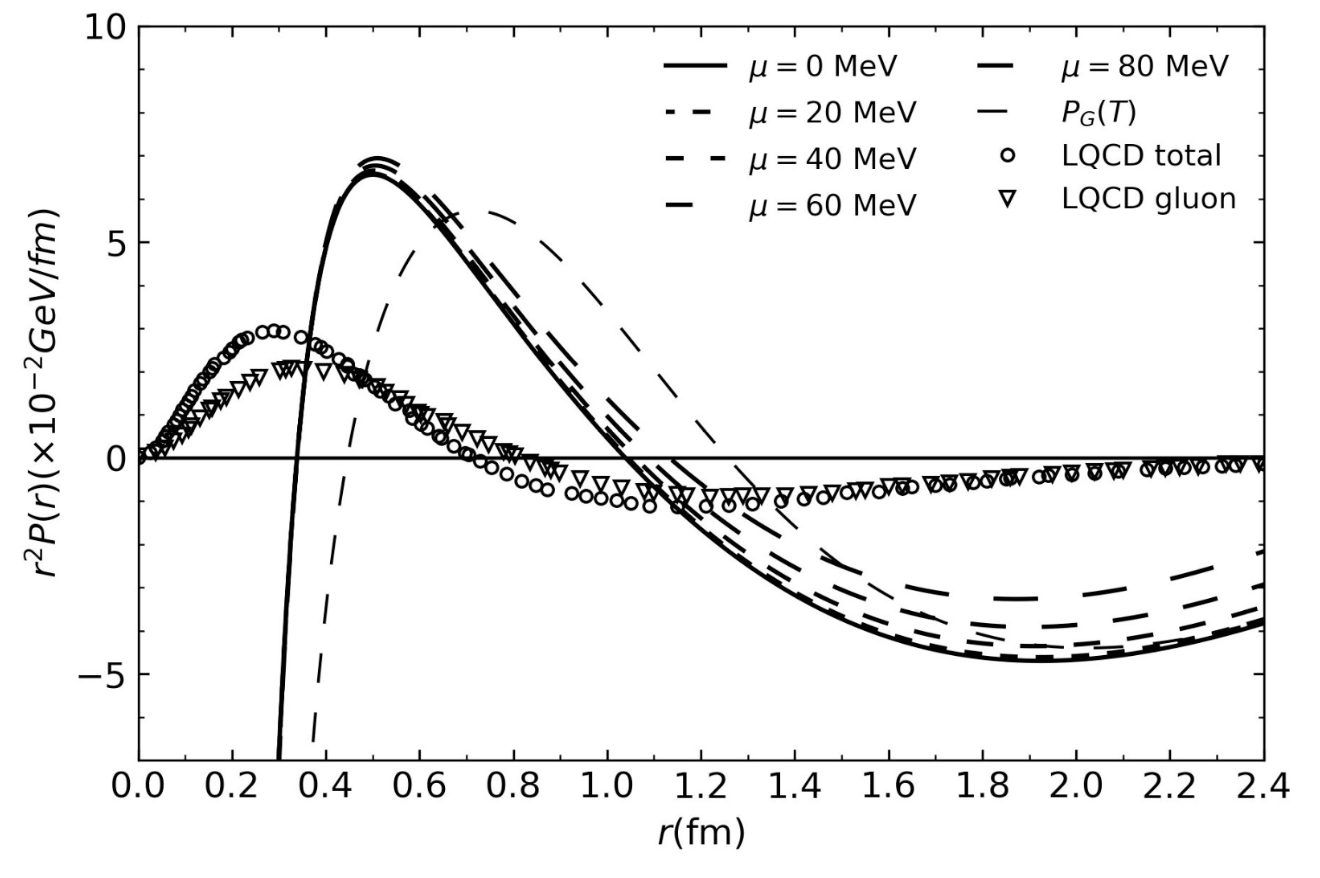
\includegraphics[width=0.58\textwidth]{./Images/MIT-BagModel.png}
    \caption[Presión radial comparada con LQCD]{\emph{Distribuciones radiales de presión \( r^2 P(r) \) obtenidas con el modelo Tsallis-MIT para distintos valores del potencial químico \( \mu \) (líneas negras), comparadas con resultados de Lattice QCD extraídos de la referencia~\cite{shanahanPressureDistributionShear2019}. Los círculos indican la presión total \( P_q \), y los triángulos invertidos la componente gluónica \( P_G \) según cálculos LQCD. Las curvas modeladas corresponden a valores de \( \mu = 0, 20, 40, 60, 80 \,\mathrm{MeV} \), y se aprecia el efecto de la densidad en el perfil de confinamiento.}}
    \label{fig: Results}
\end{wrapfigure}